\subsection{Definition}
\begin{frame}
  \frametitle{Definition}

  \begin{block}{Zweck}
  	Definition einer 1-zu-n-Abhängigkeit zwischen Objekten, damit im Fall einer Zustandsänderung eines Ojbekts alle davon abhängigen Objekte entsprechend benachrichtigt und automatisch aktualisiert werden.
  \end{block}
  	
  \begin{block}{Motivation/Ziel}
  	\begin{itemize}
  		\item asdf
  		\item asdf
  	\end{itemize}
  \end{block}
\end{frame}

\subsection{Klassendiagramm - Observer Pattern}
\begin{frame}
	\frametitle{Observer Pattern}
	\begin{itemize}
		\item Basiert auf Rollen
		\item Stellt Mechanismus zur Broadcast-Kommunikation dar
	\end{itemize}	
	
  	\begin{figure}
		\includegraphics[scale=.4]{paper/observer/observer}
	\end{figure}
\end{frame}


\subsection{Beispiel - Arbeitsvermittlung}
\begin{frame}
	\frametitle{Arbeitsvermittlung}
	\begin{itemize}
		\item 1-zu-n-Kommunikation zwischen Vermittlung und Klienten (Broadcast)
		\item Arbeitsvermittlung kennt weder Anzahl noch konkrete Klienten
		\item Klienten melden sich nur an, wenn sie daran interessiert sind.
	\end{itemize}		 
  	\begin{figure}
		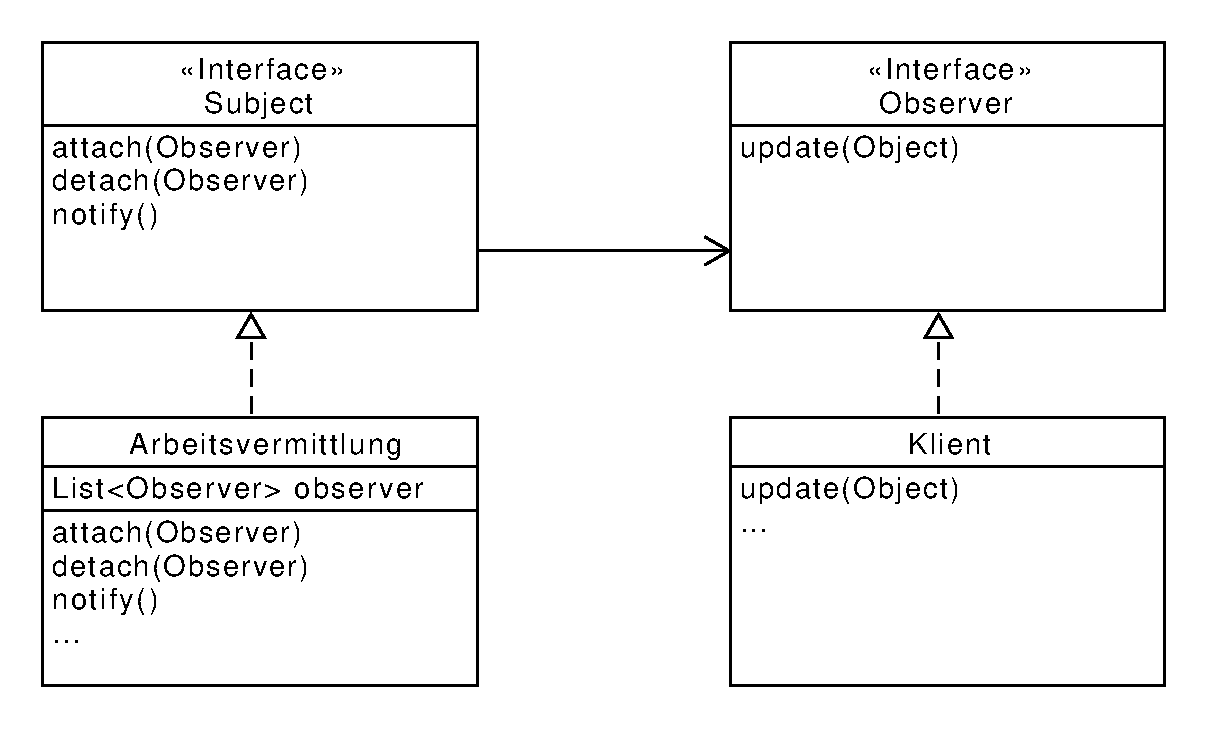
\includegraphics[scale=.4]{paper/observer/arbeitsvermittlung}
	\end{figure}
\end{frame}


\begin{frame}
\frametitle{Beispiel - Klient}
		\javacode{resources/observer_Subject_Interface.java} 
  		\javacode{resources/observer_Klient.java}	  
\end{frame}

\begin{frame}
\frametitle{Beispiel - Arbeitsvermittlung}
		\javacode{resources/observer_Observer_Interface.java}
  		\javacode{resources/observer_Arbeitsvermittlung.java}	  
\end{frame}

\subsection{Implementierungsmöglichkeiten}
\begin{frame}
\frametitle{Implementierungsmöglichkeiten}
		\begin{block}{Push Modell}
		  \begin{itemize}
		  	\item Daten nur in der update-Methode
		  	\item Zugriff auf Subject nicht erlaubt
		  	\item Subjekt muss Interesse der Observer kennen.
		  \end{itemize}
  		\end{block}
  		\begin{block}{Pull Modell}
  		 \begin{itemize}
		  	\item update-Methode ohne Parameter
		  	\item Zugriff auf Subjekt erwünscht
		  	\item Observer müssen Subject kennen
		  \end{itemize}  
  		\end{block}
  		Beides kann auch gemischt weden!
\end{frame}


\begin{frame}
\frametitle{Implementierungsmöglichkeiten}
		  \begin{block}{Observer beobachten mehrere Subects}
		  	\begin{itemize}
		  		\item Observer registriert sich bei mehreren Subjects
		  		\item Muss allerdings unterschiedlich darauf reagieren
		  		\item Lösung: erweiterung der update-Methode mit Subject
		  	\end{itemize}
		  \end{block}
		\javacode{resources/observer_erweiterung_update.java}  		
\end{frame}

\begin{frame}
\frametitle{Implementierungsmöglichkeiten}
		\begin{block}{Ausführung der Updates durch Subject}
  		 \begin{itemize}
		  	\item Weniger fehleranfällig
		  	\item Jedoch zu häufige Updates
		  \end{itemize}  
  		\end{block}		
  		\begin{block}{Ausführung der Updates durch Client}
		  \begin{itemize}
		  	\item Fehleranfälliger
		  	\item Regulierung der Updates
		  \end{itemize}
  		\end{block}
			
\end{frame}
